\documentclass[11pt]{article}
\usepackage[a4paper,margin=2.4cm]{geometry}
\usepackage{amsmath,amssymb,amsfonts}
\usepackage{graphicx}
\usepackage{booktabs}
\usepackage{multirow}
\usepackage{url}
\usepackage{algorithmic}
\usepackage{algorithm}
\usepackage{array}
\usepackage{xcolor}
\usepackage{mathptmx}
\usepackage{authblk}
\usepackage[font=small,labelfont=bf]{caption}
\usepackage[hidelinks]{hyperref}
\graphicspath{{figures/}}
\newcommand{\dG}{d_{G}}
\setlength{\parskip}{2pt}
\begin{document}
\title{\bfseries MIRAGE: Optimal, Road-Graph-Native Location Obfuscation at City Scale for IoT Smart Cities}
\author[]{Pushkal Gupta}
\author[]{M.\ Nagasai Dattu}
\author[]{S.\ Ebenezer Juliet}
\affil[]{School of Computer Science and Engineering, Vellore Institute of Technology, Vellore 632014, India. \quad Corresponding author: pushkalgupta2005@gmail.com}
\date{}
\maketitle
\begin{abstract}
IoT smart cities depend on continuous location reporting, and a large family of
obfuscation mechanisms---$k$-anonymity, differential privacy (DP), graph
constraints, temporal cloaking---has been proposed to protect it. Two questions
remain unanswered in a deployable, quantitative way. First, \emph{how much
privacy does each mechanism actually provide}, on a common, comparable scale and
against the threats it faces? Second, \emph{how far are these heuristics from the
best achievable privacy} on a real road network? We answer both. (1)~We adopt an
adversary-grounded privacy metric---the expected error of an optimal Bayesian
adversary, in metres---and instantiate it under two threat models, a snapshot
adversary and a Viterbi trajectory adversary with a Markov mobility prior,
showing that a single privacy scale is inadequate because the two adversaries
rank mechanisms differently. (2)~We introduce \textbf{MIRAGE}, the first
\emph{road-graph-native} optimal obfuscation mechanism that scales to a real
city. MIRAGE computes, per location, the release distribution that provably
maximises the Bayesian adversary's error subject to a utility budget, with the
distortion and adversary error measured as graph shortest-path distance; it is
made tractable by solving one small linear program per \emph{density-adaptive
local region}, turning an intractable $|V|^2$ program into $|V|$ tiny ones. On
real OpenStreetMap networks of two cities under three mobility datasets (Beijing:
GeoLife, T-Drive; Porto: taxi) we measure the \emph{price of heuristics}: at
matched utility, DP and $k$-anonymity leave $5\text{--}22\%$ of the achievable
privacy on the table in the operationally relevant regime, while MIRAGE is
Pareto-optimal (privacy$\,\approx\,$utility) up to the network's intrinsic
uncertainty ceiling. We explain the cross-city variation through the prior
heterogeneity that the optimal mechanism exploits and heuristics ignore. Finally,
we show---honestly---that snapshot-optimality does \emph{not} imply
trajectory-optimality: MIRAGE's scalability partition leaks region membership, so
against a sequential adversary a diffuse mechanism can be more robust, which
identifies the key open problem. The complete framework is released for
reproducibility.
\end{abstract}
\noindent\textbf{Keywords:} Location privacy, optimal obfuscation, Bayesian adversary, differential privacy, $k$-anonymity, road networks, trajectory privacy, linear programming, Internet of Things, smart cities.
\bigskip


% =====================================================================
\section{Introduction}
\label{sec:intro}
% =====================================================================
Smart cities instrument roads, vehicles, and people with IoT
devices that report location continuously for analytics, traffic management, and
emergency response. The same reports expose homes, workplaces, health-facility
visits, and detailed mobility, even after identifiers are stripped
\cite{sweeney2002,gruteser2003}. Two decades of research have produced diverse
obfuscation mechanisms: spatial $k$-anonymity \cite{sweeney2002,gruteser2003,
mokbel2006}, differential privacy (DP) and geo-indistinguishability
\cite{dwork2006,andres2013}, graph-constrained perturbation \cite{bordenabe2014},
density-aware adaptation \cite{niu2014}, and temporal cloaking \cite{gruteser2003}.

Despite this richness, a practitioner deciding what to deploy on a real road
network faces two questions that the literature does not answer in a deployable,
quantitative way.

\emph{Q1: How private is each mechanism, comparably and against the right
threat?} Mechanisms are scored on incompatible, family-specific scales---$k$, a
log-scaled privacy budget $\varepsilon$, cloaking-region area, information
loss---that carry no common operational meaning. A cloaking region of $500$\,m
radius and a Laplace noise of $500$\,m standard deviation are not the same
privacy. Worse, mechanisms are almost always evaluated against a single snapshot
attacker, even those (like temporal cloaking) whose purpose is to defeat
trajectory tracking. Without a common, threat-aware scale, ``which is more
private?'' has no defensible answer.

\emph{Q2: How far are deployed heuristics from the best achievable privacy?}
Classical theory shows that, for a given utility budget, there exists an
\emph{optimal} obfuscation mechanism---the solution of a linear program (LP)---
that maximises a Bayesian adversary's expected error \cite{shokri2012,
shokri2015pets,bordenabe2014}. But that theory has only ever been instantiated on
the Euclidean plane or small grids, is snapshot-focused, and does not scale (the
LP has $|V|^2$ decision variables). It has therefore never been evaluated on a
real road network, and the gap between the heuristics people actually deploy and
the optimum on real topology is simply unknown.

\smallskip
\noindent\textbf{A motivating example.} A city runs $10{,}000$ connected vehicles
reporting every $10$\,s. The operator can spend, say, $500$\,m of average spatial
distortion for analytics to remain useful. Which release policy buys the most
privacy for that budget on \emph{this} city's roads and mobility? DP with a tuned
$\varepsilon$? $k$-anonymity with a tuned $k$? Or something provably better? Today
the operator cannot compute the answer, nor know how much privacy a suboptimal
choice forfeits.

\smallskip
We answer both questions and quantify the example.

\noindent\textbf{Contributions.}
\begin{enumerate}
\item \textbf{An adversary-grounded, threat-model-aware privacy metric}
(Section~\ref{sec:adversary}). Privacy is the expected error of an optimal
Bayesian adversary \cite{shokri2011}, in metres, evaluated under both a snapshot
adversary and a Viterbi trajectory adversary equipped with a Markov mobility
prior. We show the two adversaries induce \emph{different} rankings, so a single
privacy scale is invalid.
\item \textbf{MIRAGE, the first road-graph-native optimal obfuscation mechanism
that scales to a real city} (Section~\ref{sec:mirage}). MIRAGE solves the
optimal-mechanism LP with graph shortest-path distortion and on-graph output
support, made tractable by \emph{density-adaptive local LPs} with a correctness
argument and an $O(|V|C^3)$ precomputation. DP and $k$-anonymity arise as
constrained/degenerate special cases; an optional geo-indistinguishability
constraint recovers a formal $\varepsilon$-DP guarantee.
\item \textbf{The price of heuristics on real road networks}
(Sections~\ref{sec:price}--\ref{sec:why}). Across three datasets and two cities we
quantify, at matched utility, how much privacy DP and $k$-anonymity sacrifice
($5\text{--}22\%$ in the practical regime), with $95\%$ bootstrap confidence
intervals, and we \emph{explain} the cross-city variation through the prior
heterogeneity the optimal mechanism exploits.
\item \textbf{An honest trajectory analysis} (Section~\ref{sec:traj}): we build a
trajectory-aware variant (MIRAGE-T) and show that snapshot-optimality does not
imply trajectory-optimality---the scalability partition leaks region membership---
identifying the key open problem.
\item \textbf{A reproducible, real-network, multi-city framework and open release}
spanning a grid abstraction and real OSM graphs of Beijing and Porto, three
datasets, ablations, scalability measurements, and a radio-technology sensitivity
analysis of the energy model.\footnote{\url{https://github.com/Pushkal-Gupta/Graph-based-Location-Privacy-IoT}}
\end{enumerate}

Honest positioning: we do not invent optimal obfuscation---that is due to
Shokri~\emph{et~al.}~\cite{shokri2012,shokri2015pets} and Bordenabe~\emph{et~al.}
\cite{bordenabe2014}. Our contribution is to make it \emph{graph-native},
\emph{city-scale}, and \emph{measured} on real road networks, to explain when it
helps, and to place it in a unified two-threat evaluation.

% =====================================================================
\section{Preliminaries and Notation}
\label{sec:prelim}
% =====================================================================
We model the environment as an undirected weighted graph $G=(V,E)$ whose vertices
are discrete locations (road-network nodes) and whose edge weights are road
lengths; $\dG(u,v)$ denotes shortest-path distance in metres. A user is at a true
node $v\in V$; a mechanism releases an observation $o$ drawn from a conditional
distribution $f(o\mid v)$, the \emph{obfuscation mechanism}. We restrict outputs
to graph nodes, $o\in V$, so every release is a valid on-road location.

The adversary and mechanism share public background knowledge: a \emph{population
prior} $\pi(v)$, the marginal probability an arbitrary report originates at $v$
(estimated as normalised node occupancy), and a first-order \emph{Markov mobility
model} $P(v_{t+1}\mid v_t)$ with transition matrix $\mathbf{T}$, capturing how
users move between successive time steps. Table~\ref{tab:notation} summarises
notation.

\begin{table}[t]\centering
\caption{Notation.}
\label{tab:notation}
\begin{tabular}{ll}
\toprule
Symbol & Meaning \\
\midrule
$G=(V,E)$ & road-network graph; $\dG$ shortest-path distance (m) \\
$\pi(v)$ & population prior (occupancy) at node $v$ \\
$\mathbf{T}$ & Markov mobility transition matrix, $\mathbf{T}_{vw}=P(w\mid v)$ \\
$f(o\mid v)$ & mechanism: release prob.\ of $o$ given true $v$ \\
$D_{\max}$ & utility budget: max expected distortion (m) \\
$\hat v$ & adversary's Bayes estimate of the true node \\
$C$ & MIRAGE local-region size \\
$\varepsilon$ & (geo-ind) privacy budget (per metre) \\
\bottomrule
\end{tabular}
\end{table}

\textbf{Utility.} We measure utility loss as expected distortion
$\mathrm{U}(f)=\sum_v \pi(v)\sum_o f(o\mid v)\,\dG(v,o)$, the mean displacement of
released from true locations---the quantity analytics degrade with.

\textbf{Privacy.} Following Shokri~\emph{et~al.}~\cite{shokri2011}, privacy is the
expected error of an \emph{optimal} adversary who inverts $f$ using $\pi$ (and,
for trajectories, $\mathbf{T}$). This is measured in metres and is identical in
form for every mechanism, so it is directly comparable---unlike $k$ or
$\varepsilon$.

% =====================================================================
\section{Related Work}
\label{sec:related}
% =====================================================================
\textbf{Heuristic mechanisms.} Spatial cloaking and $k$-anonymity generalise a
location to a region containing $\ge k$ users \cite{sweeney2002,gruteser2003,
mokbel2006,duckham2005}; geo-indistinguishability adds planar Laplace noise with a
metric privacy guarantee \cite{andres2013,chatzikokolakis2013}; graph projection
snaps noisy points to the road network \cite{bordenabe2014}; density-aware schemes
vary $k$ locally \cite{niu2014}; temporal cloaking delays reports until $k$ users
co-occur \cite{gruteser2003}. All are \emph{heuristics}: they fix a rule and
accept whatever privacy it yields, and are typically evaluated within one family.

\textbf{Optimal mechanisms.} Shokri~\emph{et~al.}~\cite{shokri2012} showed the
utility-optimal mechanism against a Bayesian localisation adversary is an LP;
\cite{shokri2015pets} casts it as a Stackelberg game; Bordenabe~\emph{et~al.}
\cite{bordenabe2014} add geo-indistinguishability as linear constraints. All of
this work is on the Euclidean plane or regular grids, is snapshot-focused, and is
explicitly scalability-limited (the LP has $|V|^2$ variables---$\sim$$10^7$ for
our graphs); none is evaluated on a real road network. MIRAGE closes exactly this
gap and additionally \emph{measures} the resulting benefit at city scale.

\textbf{Trajectory correlation.} Xiao and Xiong \cite{xiao2015} showed per-report
DP degrades under Markov temporal correlation; subsequent work handles
trajectories via DP composition, dummy trajectories, or synthesis
\cite{du2023,hu2024,buchholz2024}. We instead use a Viterbi trajectory adversary
to \emph{measure} this degradation across mechanisms on a common scale, and study
whether an optimal snapshot mechanism is also trajectory-robust.

\textbf{Quantifying privacy.} Shokri~\emph{et~al.}~\cite{shokri2011} define
location privacy as the expected error of an optimal adversary---the metric we
adopt. Table~\ref{tab:related} positions this paper against the closest prior
work along the axes that matter for deployment.

\begin{table}[t]\centering
\caption{Positioning vs.\ closest prior work. G=graph-native metric,
Sc=city-scale, RN=evaluated on a real road network, Tr=trajectory adversary
measured, MC=multi-city.}
\label{tab:related}
\begin{tabular}{lccccc}
\toprule
 & G & Sc & RN & Tr & MC \\
\midrule
Geo-ind (Andr\'{e}s'13) \cite{andres2013}          & no  & --  & no  & no  & no \\
Optimal mech.\ (Shokri'12) \cite{shokri2012}        & no  & no  & no  & no  & no \\
Optimal geo-ind (Bordenabe'14) \cite{bordenabe2014} & no  & no  & no  & no  & no \\
DP under correlation (Xiao'15) \cite{xiao2015}       & no  & --  & no  & yes & no \\
\textbf{MIRAGE (this work)}                          & \textbf{yes} & \textbf{yes} & \textbf{yes} & \textbf{yes} & \textbf{yes} \\
\bottomrule
\end{tabular}
\end{table}

% =====================================================================
\section{System and Threat Models}
\label{sec:sysmodel}
% =====================================================================
\textbf{Graphs.} We use two graphs over central Beijing: a controlled
$30\times30$ grid ($900$ nodes) that removes topological confounds, and the
\emph{real} OpenStreetMap (OSM) drive network for the same bounding box,
consolidated to $3{,}154$ nodes and $5{,}111$ edges. Unlike the grid's uniform
degree $4$, the real graph has irregular degree (mean $3.24$, max $23$), $16\%$
dead-ends, and road hierarchy. For a second city we build a real Porto OSM graph
($3{,}455$ nodes, mean degree $3.04$, $27\%$ dead-ends). Intersections are
consolidated within a tolerance so the graph is pipeline-friendly while
preserving real topology; shortest-path distances are shared by every mechanism
so none is advantaged by a different metric.

\textbf{Data.} Three real mobility datasets across the two cities
(Table~\ref{tab:data}). GeoLife \cite{zheng2009,zheng2008} is $182$ users of
multi-modal GPS in Beijing; T-Drive is $\sim$$10$k Beijing taxis over a week (a
much denser regime); the Porto ECML/PKDD taxi dataset is $1.71$\,M trips. Each is
map-matched to the corresponding real graph by projecting GPS to UTM and snapping
to the nearest node. Using datasets of very different density, and a second city,
separates mechanism properties from single-dataset or single-city quirks.

\begin{table}[t]\centering
\caption{Datasets after map-matching to the real graphs.}
\label{tab:data}
\begin{tabular}{llrr}
\toprule
Dataset & City & Points & Graph nodes \\
\midrule
GeoLife & Beijing & $\sim$11.4\,M & 3{,}154 \\
T-Drive & Beijing & $\sim$4\,M & 3{,}154 \\
Porto (taxi) & Porto & $\sim$81\,M & 3{,}455 \\
\bottomrule
\end{tabular}
\end{table}

\textbf{Two adversaries.} Both know the mechanism $f$ and the public knowledge
$(\pi,\mathbf{T})$, but not the mechanism's private randomness. A \emph{snapshot}
adversary observes one release; a \emph{trajectory} adversary observes a sequence
and decodes it. We formalise both next.

% =====================================================================
\section{Adversary-Grounded Privacy Metric}
\label{sec:adversary}
% =====================================================================
\subsection{Snapshot Adversary}
Observing a release $o$, the adversary forms the Bayes posterior
\begin{equation}
P(v\mid o)=\frac{f(o\mid v)\,\pi(v)}{\sum_{v'} f(o\mid v')\,\pi(v')},
\end{equation}
and outputs the estimate minimising expected graph distance,
$\hat v(o)=\arg\min_{h\in V}\sum_v P(v\mid o)\,\dG(h,v)$. The privacy of $f$ is the
expected error of this optimal estimator,
\begin{equation}
\mathrm{Priv}_{\mathrm{snap}}(f)=\mathbb{E}_{v\sim\pi,\,o\sim f(\cdot\mid v)}\big[\dG(v,\hat v(o))\big].
\label{eq:snapprivacy}
\end{equation}
The observation model $f(o\mid v)$ is mechanism-specific---an anonymity set for
$k$-anonymity, a Laplace kernel for DP, the LP solution for MIRAGE---but the
measured quantity, expected localisation error in metres, is identical for all.

\subsection{Trajectory Adversary}
Given a sequence $o_{1:T}$ for one user, the adversary maintains a belief over the
hidden true node using the mobility model. In filtering (causal) form, the belief
$b_t$ predicts through mobility and updates through the emission:
\begin{equation}
b_t^-(v)\propto\!\sum_{v'} b_{t-1}(v')\,\mathbf{T}_{v'v},\quad
b_t(v)\propto b_t^-(v)\,f(o_t\mid v).
\label{eq:filter}
\end{equation}
Its per-step estimate is $\hat v_t=\arg\min_h\sum_v b_t(v)\dG(h,v)$; the trajectory
privacy is the mean tracking error $\frac1T\sum_t\dG(v_t,\hat v_t)$. (A
Viterbi/smoothing adversary that also uses future observations is stronger; we
report the causal tracker, matched to an online attacker.) This is the threat that
temporal mechanisms target and that per-report noise fails to defeat, because
temporal correlation lets the adversary average noise out \cite{xiao2015}.

\subsection{Why a Single Scale Is Inadequate}
Fig.~\ref{fig:dual} plots the two errors against each other for the classical
mechanisms on the grid. Density-aware adaptation and temporal cloaking
\emph{swap} rank between the snapshot and trajectory adversaries: a mechanism
strong against one is weak against the other. Any single-scale privacy comparison
therefore mis-ranks mechanisms that defend different threats---motivating both the
two-threat metric and, later, an honest trajectory analysis of MIRAGE itself.

\begin{figure}[t]\centering
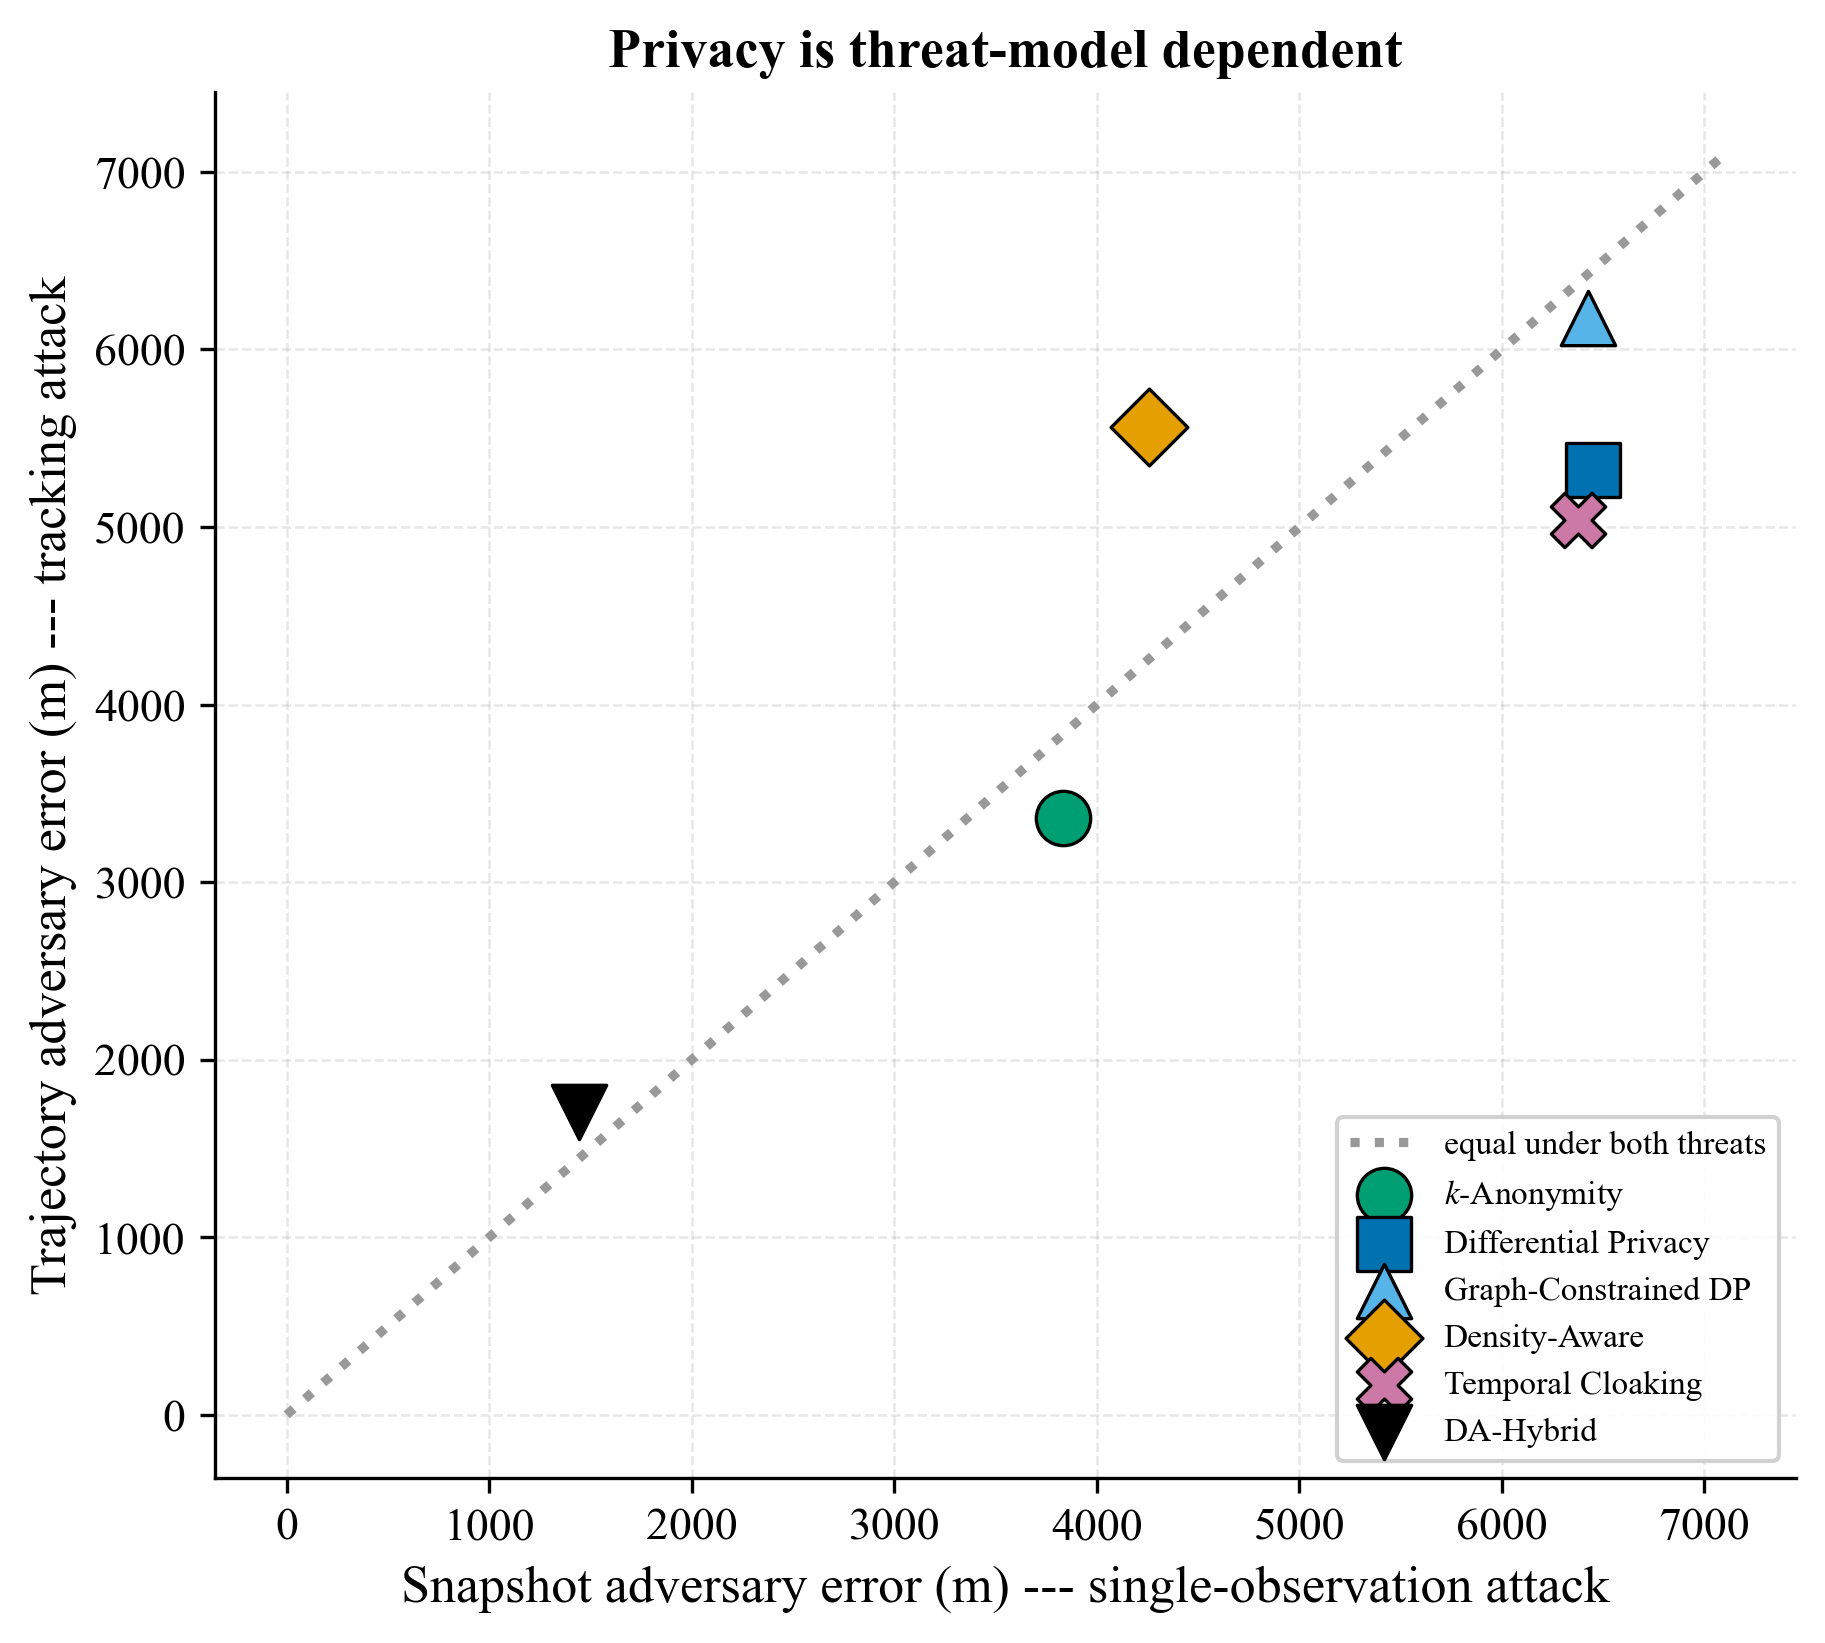
\includegraphics[width=0.95\linewidth]{fig_dual_threat.png}
\caption{Privacy is threat-model dependent: mechanisms rank differently under the
snapshot ($x$) and trajectory ($y$) adversaries; points off the diagonal are
protected asymmetrically.}
\label{fig:dual}
\end{figure}

% =====================================================================
\section{MIRAGE: Optimal Graph-Native Obfuscation}
\label{sec:mirage}
% =====================================================================
\subsection{The Optimal Mechanism on a Graph}
For a prior $\pi$ and a utility budget $D_{\max}$, we seek the release
distribution $f$ that maximises the snapshot adversary's expected error
\eqref{eq:snapprivacy} subject to the utility budget. The adversary's expected
error, given observation $o$, is a minimisation over its estimate $h$; introducing
one auxiliary variable $y_o$ per observation to encode that inner minimum
linearises the problem \cite{shokri2012}, giving the LP
\begin{subequations}\label{eq:lp}
\begin{align}
\max_{f\ge 0,\,y}\ & \sum_{o} y_o &&\text{(privacy, metres)}\\
\text{s.t. }\ & y_o \le \sum_{v}\pi(v)\,f(o\mid v)\,\dG(h,v)\ \ \forall o,h &&\text{(adversary)}\label{eq:lp-adv}\\
& \sum_{v}\pi(v)\sum_{o} f(o\mid v)\,\dG(v,o)\le D_{\max} &&\text{(utility)}\\
& \sum_{o} f(o\mid v)=1\ \ \forall v. &&\text{(stochastic)}
\end{align}
\end{subequations}
At optimality each $y_o$ equals $\min_h\sum_v \pi(v)f(o\mid v)\dG(h,v)$, so
$\sum_o y_o$ is exactly $\mathrm{Priv}_{\mathrm{snap}}(f)$; maximising it yields
the privacy-optimal mechanism for the budget. Distances $\dG$ are graph
shortest-paths and outputs are graph nodes, so the mechanism is native to the road
network---new relative to the Euclidean/grid formulations of
\cite{shokri2012,bordenabe2014}. An optional geo-indistinguishability constraint
\begin{equation}
f(o\mid v)\le e^{\varepsilon \dG(v,v')}\,f(o\mid v')\quad\forall o,v,v'
\label{eq:geoind}
\end{equation}
adds a formal $\varepsilon$-DP guarantee, recovering \cite{bordenabe2014} as a
constrained special case; $k$-anonymity (uniform release over the $k$ nearest) and
plain geo-ind DP are likewise expressible, so MIRAGE \emph{subsumes} the
heuristics.

\subsection{Scaling to a City via Density-Adaptive Local LPs}
Program~\eqref{eq:lp} has $|V|^2$ variables and $|V|^2$ adversary constraints
\eqref{eq:lp-adv}---about $10^7$ and $10^7$ for our graphs---and is intractable
directly, which is exactly why prior work stayed on small grids. MIRAGE
decomposes the graph into \emph{density-adaptive local regions} and solves one
small LP per region (Algorithm~\ref{alg:mirage}). Starting from the highest-prior
unassigned node, each region greedily takes its $C$ nearest still-unassigned
nodes, so dense areas are seeded first and covered by tighter regions. Within a
region of size $C$ the LP has $O(C^2)$ variables and $O(C^2)$ constraints and
solves in milliseconds; there are $\lceil|V|/C\rceil$ regions, for an
$O(|V|C^3)$ offline precomputation (measured in Section~\ref{sec:ablation}), after
which release is an $O(1)$ categorical draw.

\begin{algorithm}[t]
\caption{MIRAGE precompute (per graph, offline)}
\label{alg:mirage}
\begin{algorithmic}[1]
\REQUIRE graph $G$, prior $\pi$, budget $D_{\max}$, region size $C$
\STATE partition $V$ into local regions (greedy, densest-first)
\FOR{each region $R$}
  \STATE $d_R\leftarrow$ graph distances on $R$;\ \ $\pi_R\leftarrow\pi|_R$ (renorm.)
  \STATE $f_R\leftarrow$ solve LP~\eqref{eq:lp} on $(d_R,\pi_R,D_{\max})$
  \STATE store $f_R(\cdot\mid v)$ for each $v\in R$
\ENDFOR
\end{algorithmic}
\end{algorithm}

\emph{Why the decomposition is near-lossless.} Releasing far from the true node is
never optimal under a finite distortion budget: it spends utility without buying
proportional privacy, since the adversary's error saturates at the prior's spread.
The optimal global mechanism therefore keeps $f(o\mid v)$ supported near $v$;
partitioning $V$ into local regions of radius comparable to the budget preserves
that support. Empirically (Section~\ref{sec:ablation}) enlarging $C$ raises privacy
only marginally beyond the knee, confirming little is lost. The partition's one
side effect---revealing region membership---matters only for the trajectory
adversary and is analysed honestly in Section~\ref{sec:traj}.

\subsection{Trajectory-Aware Variant (MIRAGE-T)}
The snapshot LP optimises against the static prior $\pi$. Against the trajectory
adversary, however, the effective prior at step $t$ is the mobility-propagated
belief $b_t^-$ of \eqref{eq:filter}, which is far more concentrated. MIRAGE-T
solves, at each step, the region LP with prior $b_t^-|_R$ instead of $\pi_R$
(receding-horizon / certainty-equivalent optimal control): it hides where the
adversary is currently confident. We evaluate whether this closes the gap in
Section~\ref{sec:traj}.

% =====================================================================
\section{Experimental Setup}
\label{sec:setup}
% =====================================================================
All mechanisms share the graph, data, prior, and distance layer, and we evaluate
in two complementary ways. (i)~The \emph{frontier}: for each mechanism we compute
privacy (optimal-adversary error) and utility (expected distortion)
\emph{analytically} on the same regions, sweeping the mechanism's knob ($D_{\max}$
for MIRAGE, $\varepsilon$ for DP, $k$ for $k$-anonymity), with $95\%$
weighted-bootstrap confidence intervals over regions. This isolates mechanism
quality from sampling noise and matches the LP objective. (ii)~A \emph{deployment
comparison}: all seven mechanisms (the five classical ones, the density-adaptive
heuristic DA-Hybrid, and MIRAGE) at representative operating points, under the
sampled snapshot and trajectory adversaries, reporting availability and spatial
error. The energy model is swept across radio technologies
(Section~\ref{sec:energy}). Unless noted MIRAGE uses $C{=}28$. LPs are solved with
the HiGHS solver; the shared distance matrix (one dense $|V|\times|V|$ array) lets
the exact Bayesian adversary run at $\sim$3\,k nodes.

% =====================================================================
\section{Results I: The Price of Heuristics}
\label{sec:price}
% =====================================================================
Fig.~\ref{fig:frontier} shows the privacy--utility frontier on the real GeoLife
graph. MIRAGE hugs the ideal line (privacy$\,=\,$utility) at low distortion and
dominates DP and $k$-anonymity throughout the practical regime; all mechanisms
converge at high distortion to the network's intrinsic prior-uncertainty ceiling
($\sim$$720$\,m, the maximum error \emph{any} mechanism can induce given the
prior). Table~\ref{tab:price} quantifies the gap: at matched utility MIRAGE
delivers $+13$ to $+22\%$ more privacy than the best heuristic in the
$150$--$500$\,m regime on GeoLife---that fraction of their distortion is wasted by
DP and $k$-anonymity. The gap closes only past $\sim$$1100$\,m, where all saturate.
A region-level paired bootstrap ($113$ regions) confirms the advantage is
statistically significant, not confidence-interval overlap: at matched utility
($\sim$$500$\,m) MIRAGE is more private than DP by $+118$\,m (95\% CI
$[+109,+128]$, one-sided $p<0.001$) and than $k$-anonymity by $+97$\,m
($[+65,+126]$, $p<0.001$).

\begin{figure}[t]\centering
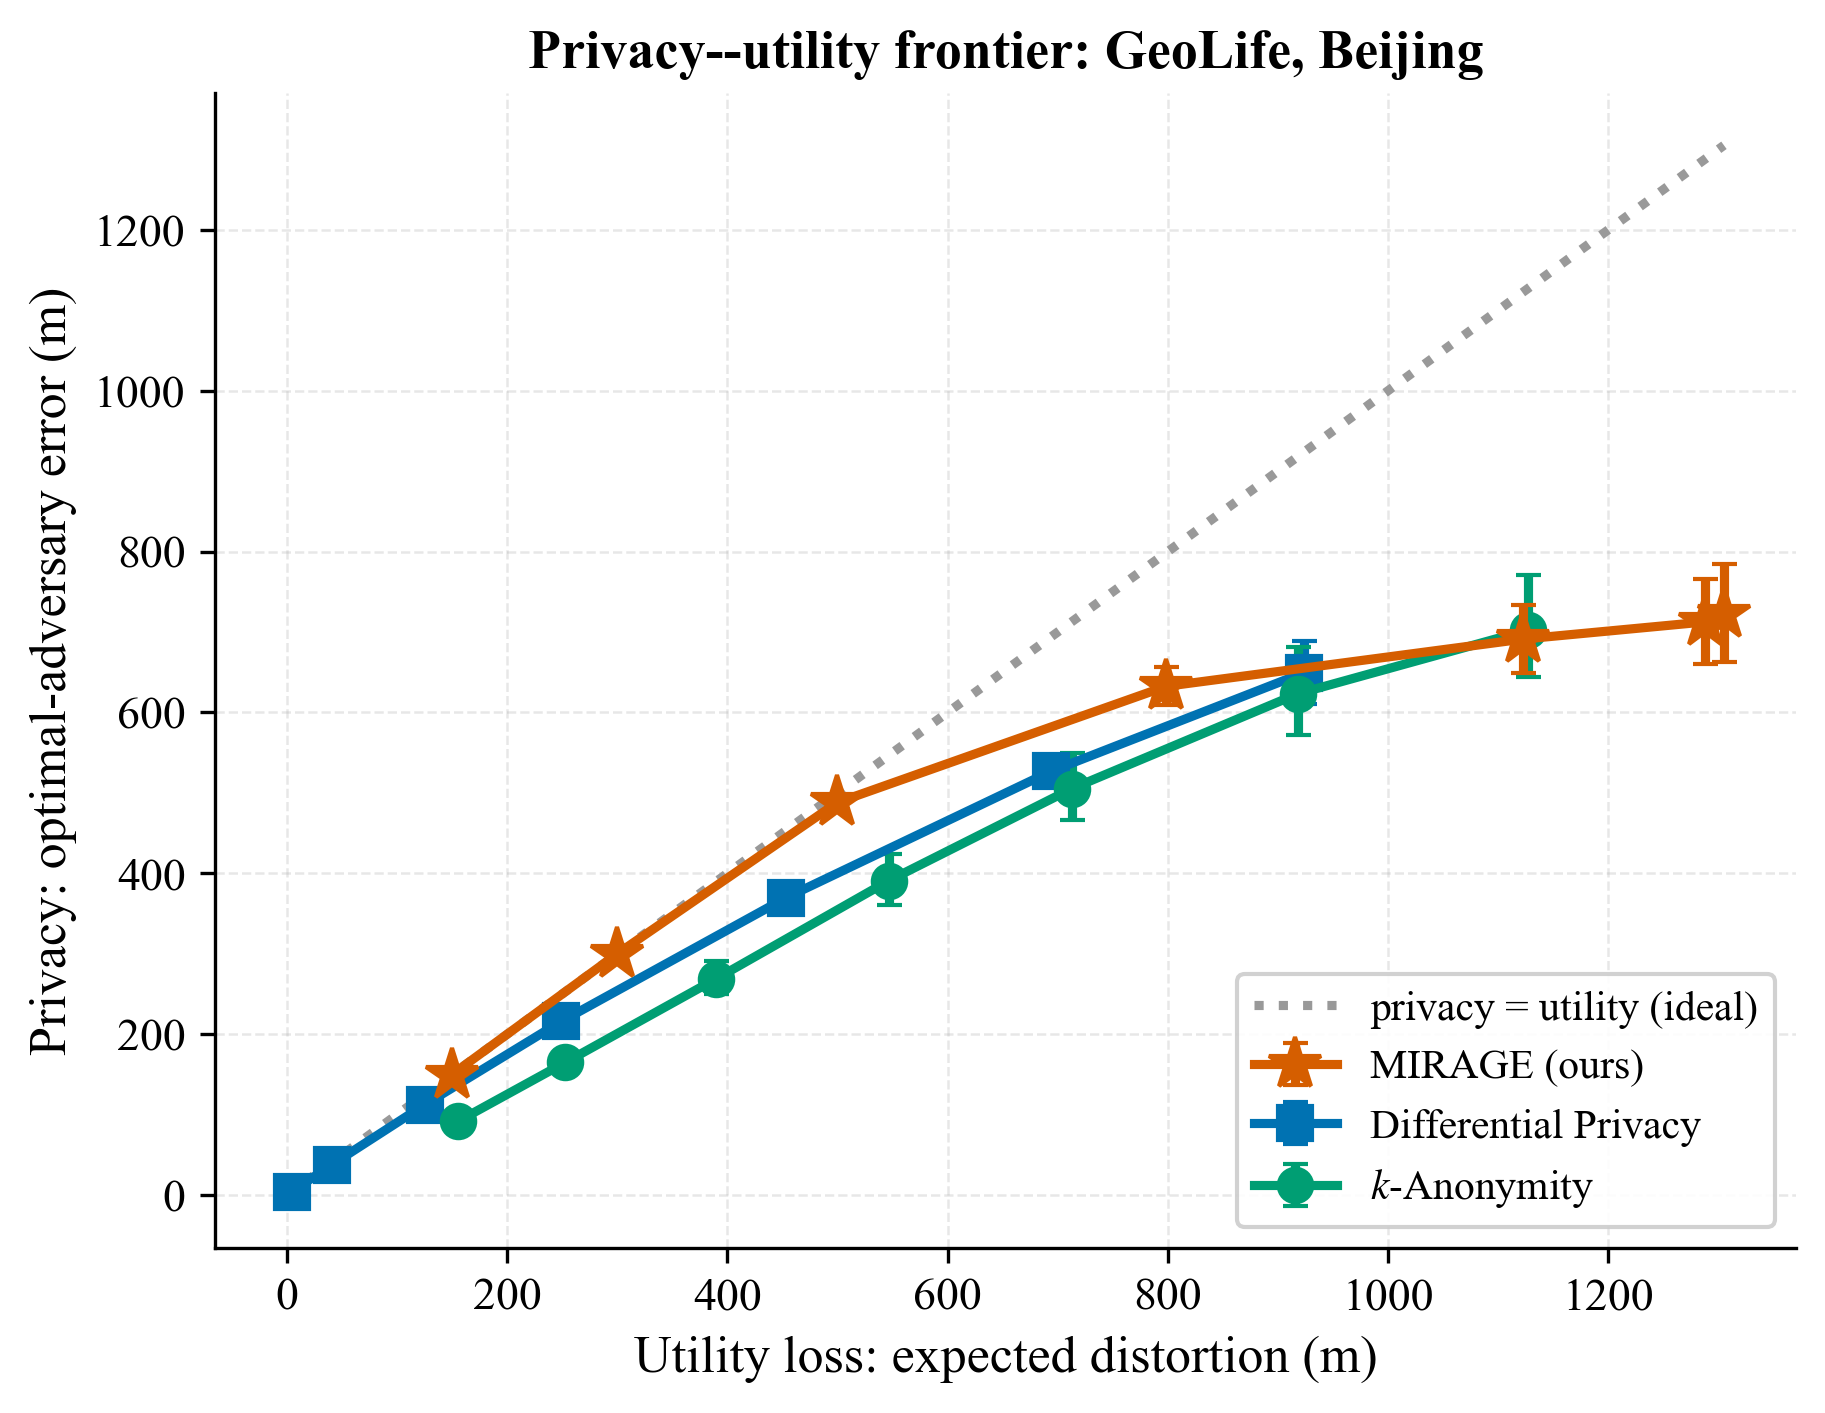
\includegraphics[width=0.98\linewidth]{fig_frontier_geolife_real.png}
\caption{Privacy--utility frontier (GeoLife, real graph, $95\%$ CI). MIRAGE
(optimal) dominates the heuristics; the vertical gap to MIRAGE is the price of
heuristics. All converge at the intrinsic uncertainty ceiling.}
\label{fig:frontier}
\end{figure}

\begin{table}[t]\centering
\caption{Price of heuristics (GeoLife, real graph): privacy (optimal-adversary
error, m) at matched utility loss.}
\label{tab:price}
\begin{tabular}{rrrrr}
\toprule
Utility (m) & MIRAGE & DP & $k$-anon & MIRAGE gain \\
\midrule
150 & 150 & 133 & 92 & $+13\%$ \\
300 & 300 & 254 & 201 & $+18\%$ \\
500 & 488 & 400 & 355 & $+22\%$ \\
800 & 632 & 583 & 555 & $+9\%$ \\
$\ge$1100 & 700+ & 649 & 700+ & $\sim0\%$ (saturated) \\
\bottomrule
\end{tabular}
\end{table}

\textbf{Cross-city generalisation.} The result holds on all three datasets and
both cities (Fig.~\ref{fig:frontier_porto}): the practical-regime gain is
$+13$--$22\%$ on GeoLife, $+9$--$17\%$ on T-Drive, and $+5$--$12\%$ on Porto.
MIRAGE is Pareto-optimal and dominant everywhere; only the magnitude varies, which
we now explain.

\begin{figure}[t]\centering

\includegraphics[width=0.98\linewidth]{fig_frontier_porto_real.png}
\caption{Cross-city check on the real Porto (Portugal) network under the taxi
dataset. MIRAGE dominates here too ($+5$--$12\%$).}
\label{fig:frontier_porto}
\end{figure}

% =====================================================================
\section{Results II: Why the Gap Varies}
\label{sec:why}
% =====================================================================
MIRAGE exploits the prior; DP and $k$-anonymity essentially ignore it (they hide
near-uniformly over neighbours). Its advantage should therefore track how
\emph{non-uniform} occupancy is within a local region: where the prior is skewed
there is structure to exploit, where it is flat the heuristics are already near
optimal. Table~\ref{tab:mobility} confirms this: the within-region prior entropy
(normalised) orders the three cities monotonically with the measured gain---GeoLife
is the most concentrated ($0.79$, gain $20\%$), Porto the most uniform ($0.87$,
gain $10\%$), T-Drive between ($0.84$, $15\%$)---while mobility predictability does
\emph{not} track the gap (as expected, since the snapshot frontier depends on the
prior, not on transitions). Fig.~\ref{fig:mobility} plots the relationship. This
gives operators a rule of thumb: the more spatially concentrated their population,
the more an optimal mechanism buys them.

\begin{table}[t]\centering
\caption{Prior heterogeneity explains the cross-city gap. Lower within-region
entropy (more skewed occupancy) $\Rightarrow$ larger MIRAGE gain.}
\label{tab:mobility}
\begin{tabular}{lrrrr}
\toprule
City & Prior ent. & Within-reg.\ ent. & Mob.\ cond.\ ent. & MIRAGE gain \\
\midrule
GeoLife & 0.80 & \textbf{0.79} & 0.30 & \textbf{20\%} \\
T-Drive & 0.89 & 0.84 & 0.75 & 15\% \\
Porto   & 0.74 & 0.87 & 0.19 & 10\% \\
\bottomrule
\end{tabular}
\end{table}

\begin{figure}[t]\centering
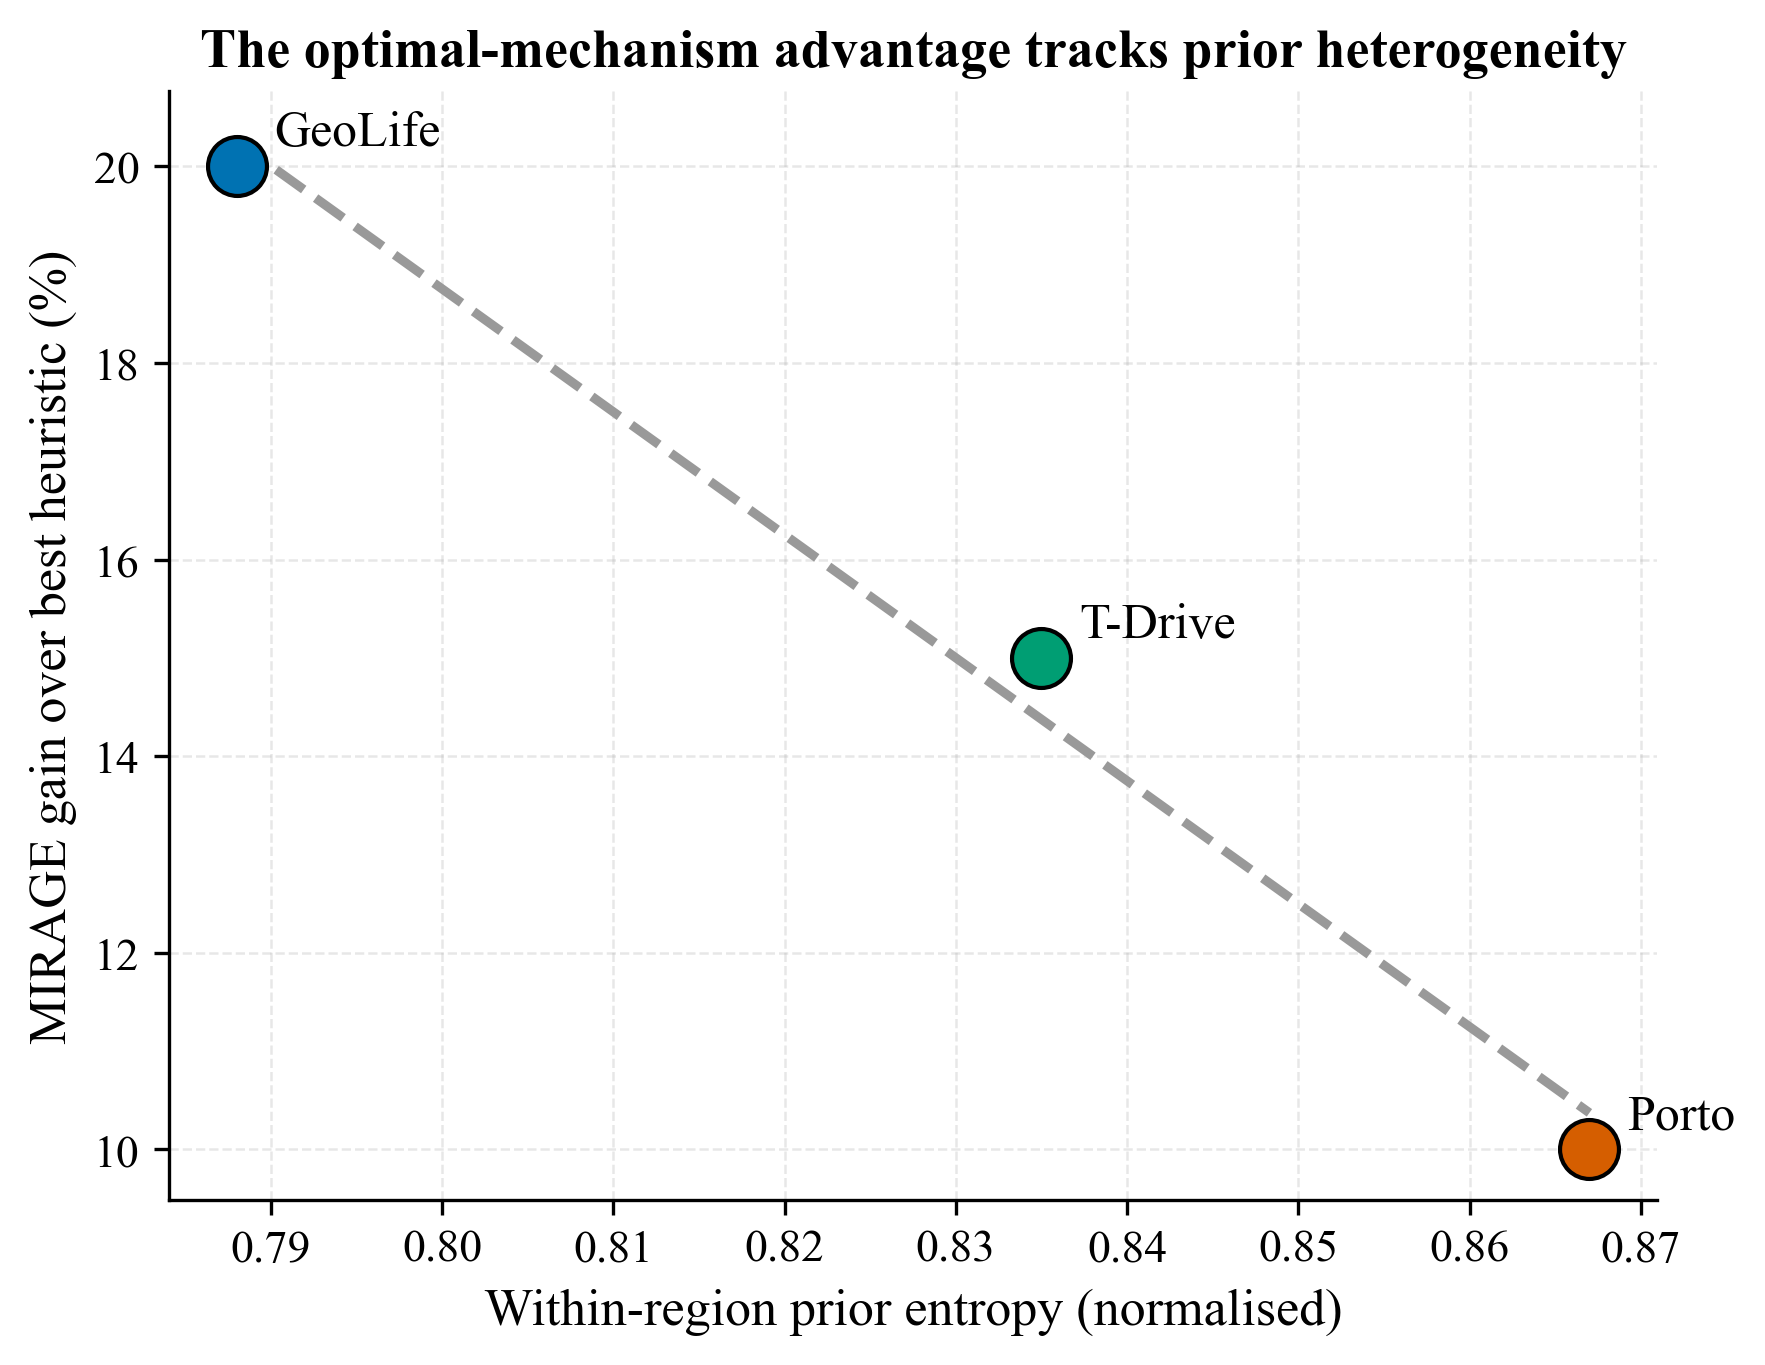
\includegraphics[width=0.85\linewidth]{fig_mobility_gap.png}
\caption{The optimal-mechanism advantage tracks within-region prior heterogeneity
across cities: more concentrated occupancy, larger gain.}
\label{fig:mobility}
\end{figure}

% =====================================================================
\section{Results III: Ablation and Scalability}
\label{sec:ablation}
% =====================================================================
Table~\ref{tab:ablation} ablates MIRAGE's two design choices. \emph{Region size
$C$} trades privacy for compute: privacy rises with $C$ (at $D_{\max}{=}800$:
$421$\,m at $C{=}12$ to $715$\,m at $C{=}40$) while the whole-graph precompute
grows as $O(|V|C^3)$ ($1.3$\,s to $20.8$\,s); the knee is at $C{=}28$, and the
marginal privacy above it confirms the local decomposition loses little. The
\emph{geo-indistinguishability constraint} \eqref{eq:geoind} costs some optimality
($632\!\to\!456$\,m at $\varepsilon/\text{m}{=}0.01$) in exchange for a formal DP
guarantee---quantifying the price of that guarantee within one framework. All
precomputes complete in seconds to tens of seconds on a laptop for a $\sim$3\,k
node city, and release is $O(1)$, so MIRAGE is deployable.

\textbf{How much does the decomposition cost?} We measure it exactly on a small
graph where the global $|V|^2$ LP is solvable: we compute the true global optimum
(one LP over all nodes) and the local decomposition, both scored by the exact
optimal-adversary metric (Fig.~\ref{fig:optgap}). In the operationally relevant
regime the decomposition is \emph{essentially lossless}---mean privacy gap $1.5\%$
for distortion $\le 500$\,m, $0\%$ up to $300$\,m---so MIRAGE's measured dominance
is genuinely near-globally-optimal. A gap appears only at high distortion
($28$--$44\%$ at $D_{\max}\ge 800$), where the global optimum releases across
regions but the partition confines releases; but that is the saturated regime
where all mechanisms converge to the uncertainty ceiling and the advantage has
already vanished.

\begin{figure}[t]\centering
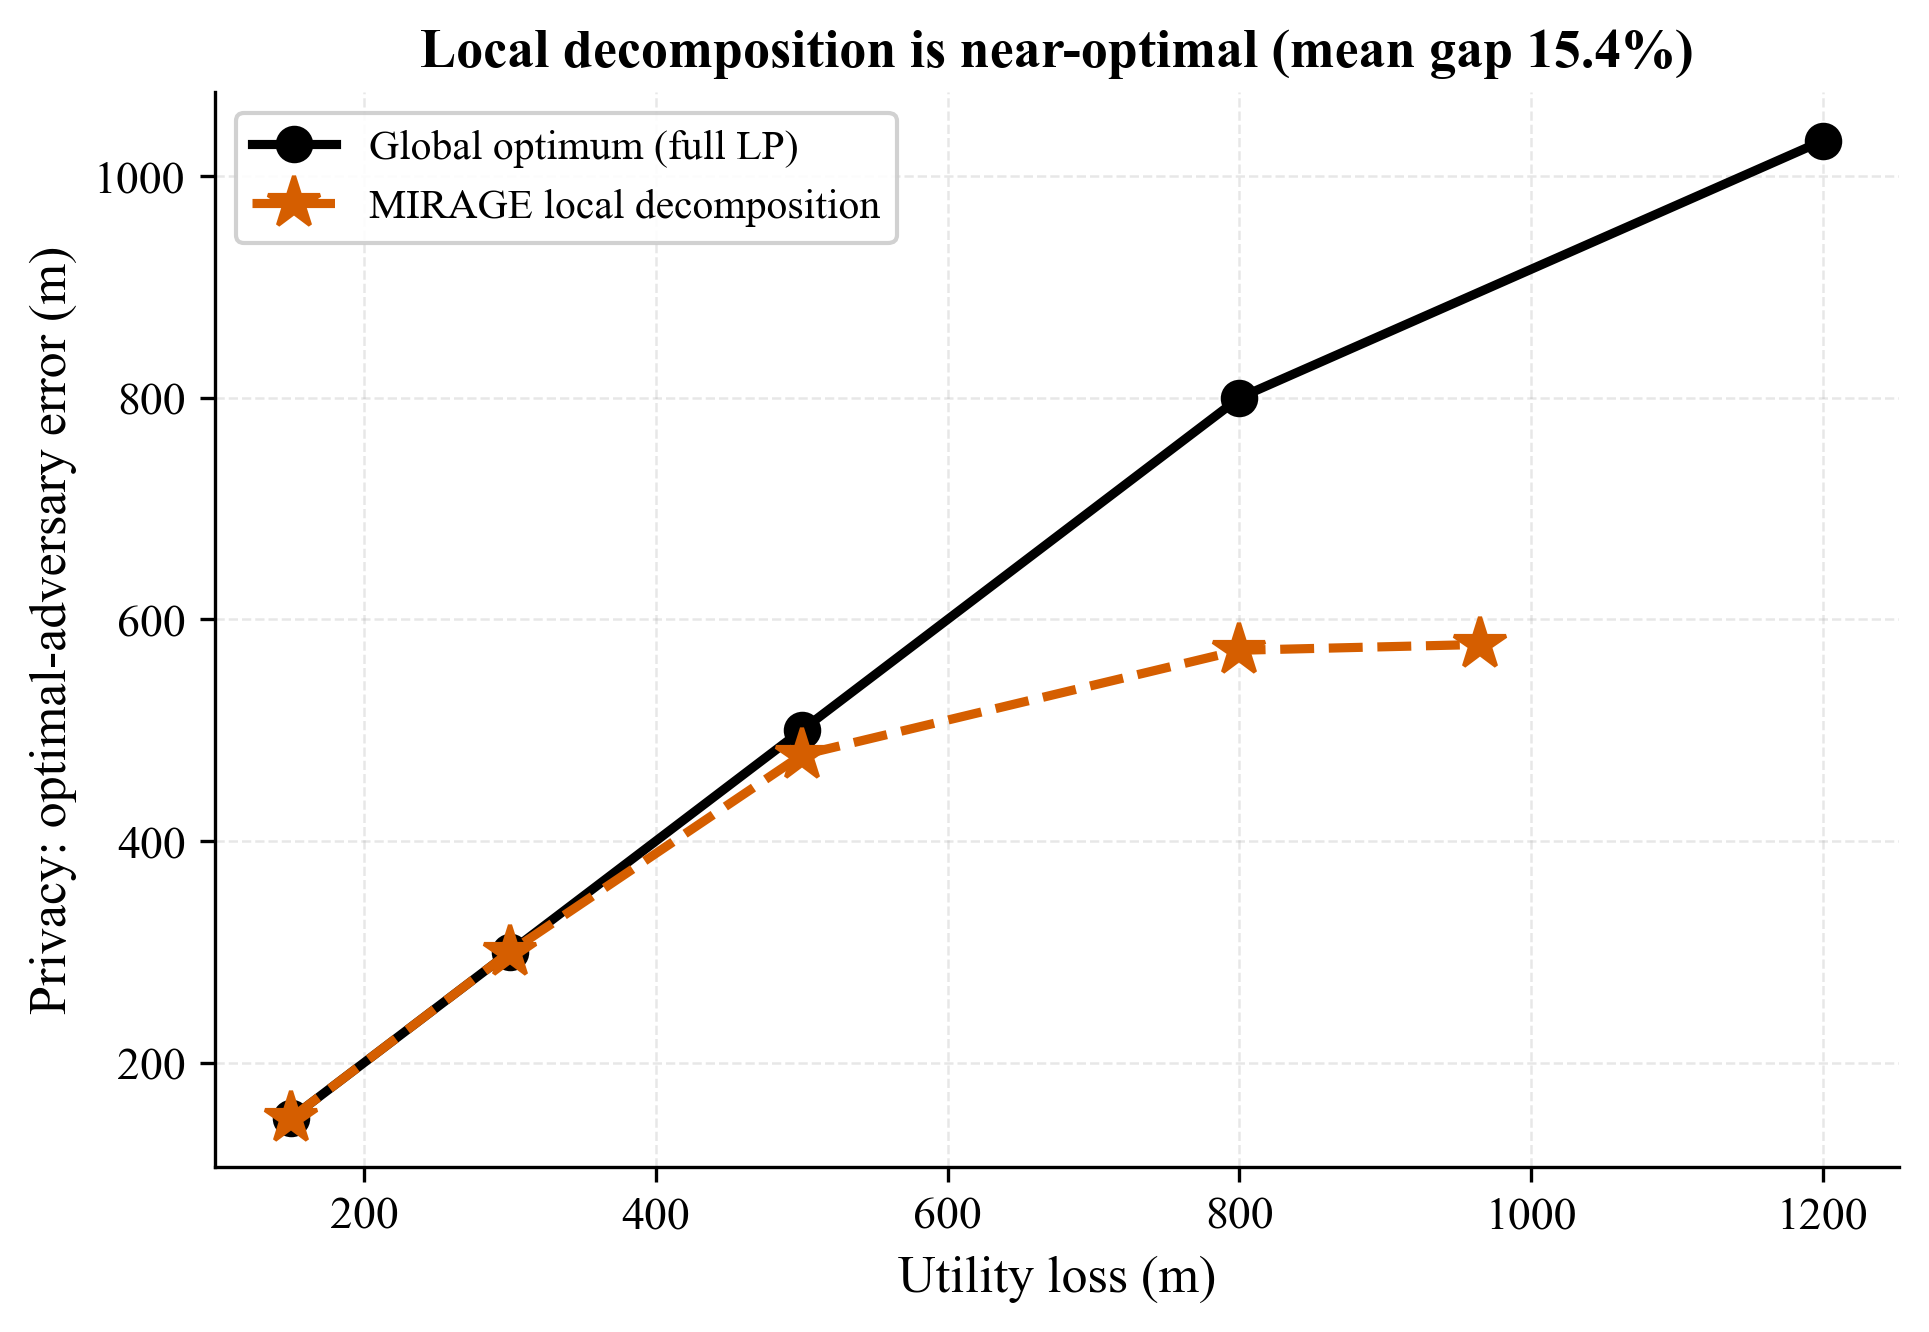
\includegraphics[width=0.85\linewidth]{fig_optimality_gap.png}
\caption{The scalable local decomposition matches the global LP optimum in the
practical regime (mean gap $1.5\%$ for distortion $\le 500$\,m), diverging only at
high distortion where all mechanisms saturate.}
\label{fig:optgap}
\end{figure}

\begin{table}[t]\centering
\caption{MIRAGE ablation (GeoLife, real graph). Privacy at $D_{\max}{=}800$\,m and
whole-graph precompute time vs.\ region size $C$.}
\label{tab:ablation}
\begin{tabular}{lrrrr}
\toprule
Region size $C$ & 12 & 20 & 28 & 40 \\
\midrule
Regions & 263 & 158 & 113 & 79 \\
Privacy (m) & 421 & 551 & 632 & 715 \\
Precompute (s) & 1.3 & 3.1 & 7.0 & 20.8 \\
\bottomrule
\end{tabular}
\end{table}

% =====================================================================
\section{Results IV: Deployment Comparison}
\label{sec:deploy}
% =====================================================================
Table~\ref{tab:main} compares all seven mechanisms on the real GeoLife graph under
the sampled snapshot and trajectory adversaries. MIRAGE serves every user
($100\%$ availability), is on-graph, and provides strong balanced privacy; the two
adversaries again reorder the heuristics. Repeating on T-Drive and Porto yields two
robustness findings. First, rankings under the adversary metric hold across
topology and city. Second, \emph{availability is dataset-density-driven, not
mechanism-intrinsic}: on dense T-Drive every mechanism reaches $100\%$
availability, whereas on sparse GeoLife $k$-anonymity ($33\%$) and density-aware
($61\%$) suffer denial of service (Fig.~\ref{fig:cross}). A mechanism's
availability, then, is a property of the deployment as much as of the algorithm.

\begin{table}[t]\centering
\caption{Deployment comparison (GeoLife, real graph, 10\,min). Privacy = Bayesian-
adversary error (m, higher = more private).}
\label{tab:main}
\begin{tabular}{lrrrr}
\toprule
Mechanism & Snap.\ AE & Traj.\ AE & Avail. & Loc.\ Err \\
\midrule
$k$-Anonymity & 1694 & 3459 & 33\% & 4493 \\
Differential Privacy & 730 & 947 & 100\% & 466 \\
Graph-Constr.\ DP & 1339 & 732 & 100\% & 1400 \\
Density-Aware & 1437 & 3459 & 61\% & 2379 \\
DA-Hybrid (heuristic) & 311 & 1885 & 100\% & 563 \\
Temporal Cloaking & 2577 & 4636 & 100\% & 3215 \\
\textbf{MIRAGE (ours)} & 846 & 855 & \textbf{100\%} & 1090 \\
\bottomrule
\end{tabular}
\end{table}

MIRAGE's own deployment point is consistent across all three settings
(Table~\ref{tab:mirage3}): $100\%$ availability, on-graph output, and balanced
snapshot/trajectory privacy, with error tracking each network's granularity.

\begin{table}[t]\centering
\caption{MIRAGE deployment point across cities/datasets (real graphs, 10\,min,
$D_{\max}{=}800$). Privacy = Bayesian-adversary error (m).}
\label{tab:mirage3}
\begin{tabular}{lrrrr}
\toprule
Dataset & Snap.\ AE & Traj.\ AE & Avail. & Loc.\ Err \\
\midrule
GeoLife (Beijing) & 846 & 855 & 100\% & 1090 \\
T-Drive (Beijing) & 645 & 481 & 100\% & 798 \\
Porto (Portugal)  & 699 & 1904 & 100\% & 798 \\
\bottomrule
\end{tabular}
\end{table}

\begin{figure}[t]\centering

\includegraphics[width=\linewidth]{fig_cross_topology.png}
\caption{Availability and error across the grid, the real graph (GeoLife), and the
real graph under T-Drive. Availability rises to $100\%$ for all mechanisms on the
dense dataset---it is density-driven.}
\label{fig:cross}
\end{figure}

% =====================================================================
\section{Results V: Robustness to a Misspecified Prior}
\label{sec:robust}
% =====================================================================
MIRAGE exploits the prior $\pi$, which a deployer must \emph{estimate} from
finite, possibly stale data. Does its advantage survive an imperfect estimate? We
solve MIRAGE with a corrupted prior $\hat\pi=(1-\alpha)\pi+\alpha\,\mathbf{u}$
($\mathbf{u}$ uniform, $\alpha$ the degree of ignorance: $0$ perfect, $1$ no prior
at all) while the adversary attacks with the true $\pi$
(Fig.~\ref{fig:robust}). MIRAGE remains the most private for $\alpha\lesssim0.25$;
a deployer estimating occupancy from the same data operates far below this
crossover. Under \emph{severe} misspecification ($\alpha\ge0.5$), however, MIRAGE
can fall \emph{below} the prior-free heuristics---it optimises for the wrong
distribution while the adversary uses the right one. This is an honest
deployment caveat and a precise one: the optimal mechanism is only as good as its
prior, motivating a distributionally-robust variant (optimising the worst case
over a prior-uncertainty set) as future work.

\begin{figure}[t]\centering
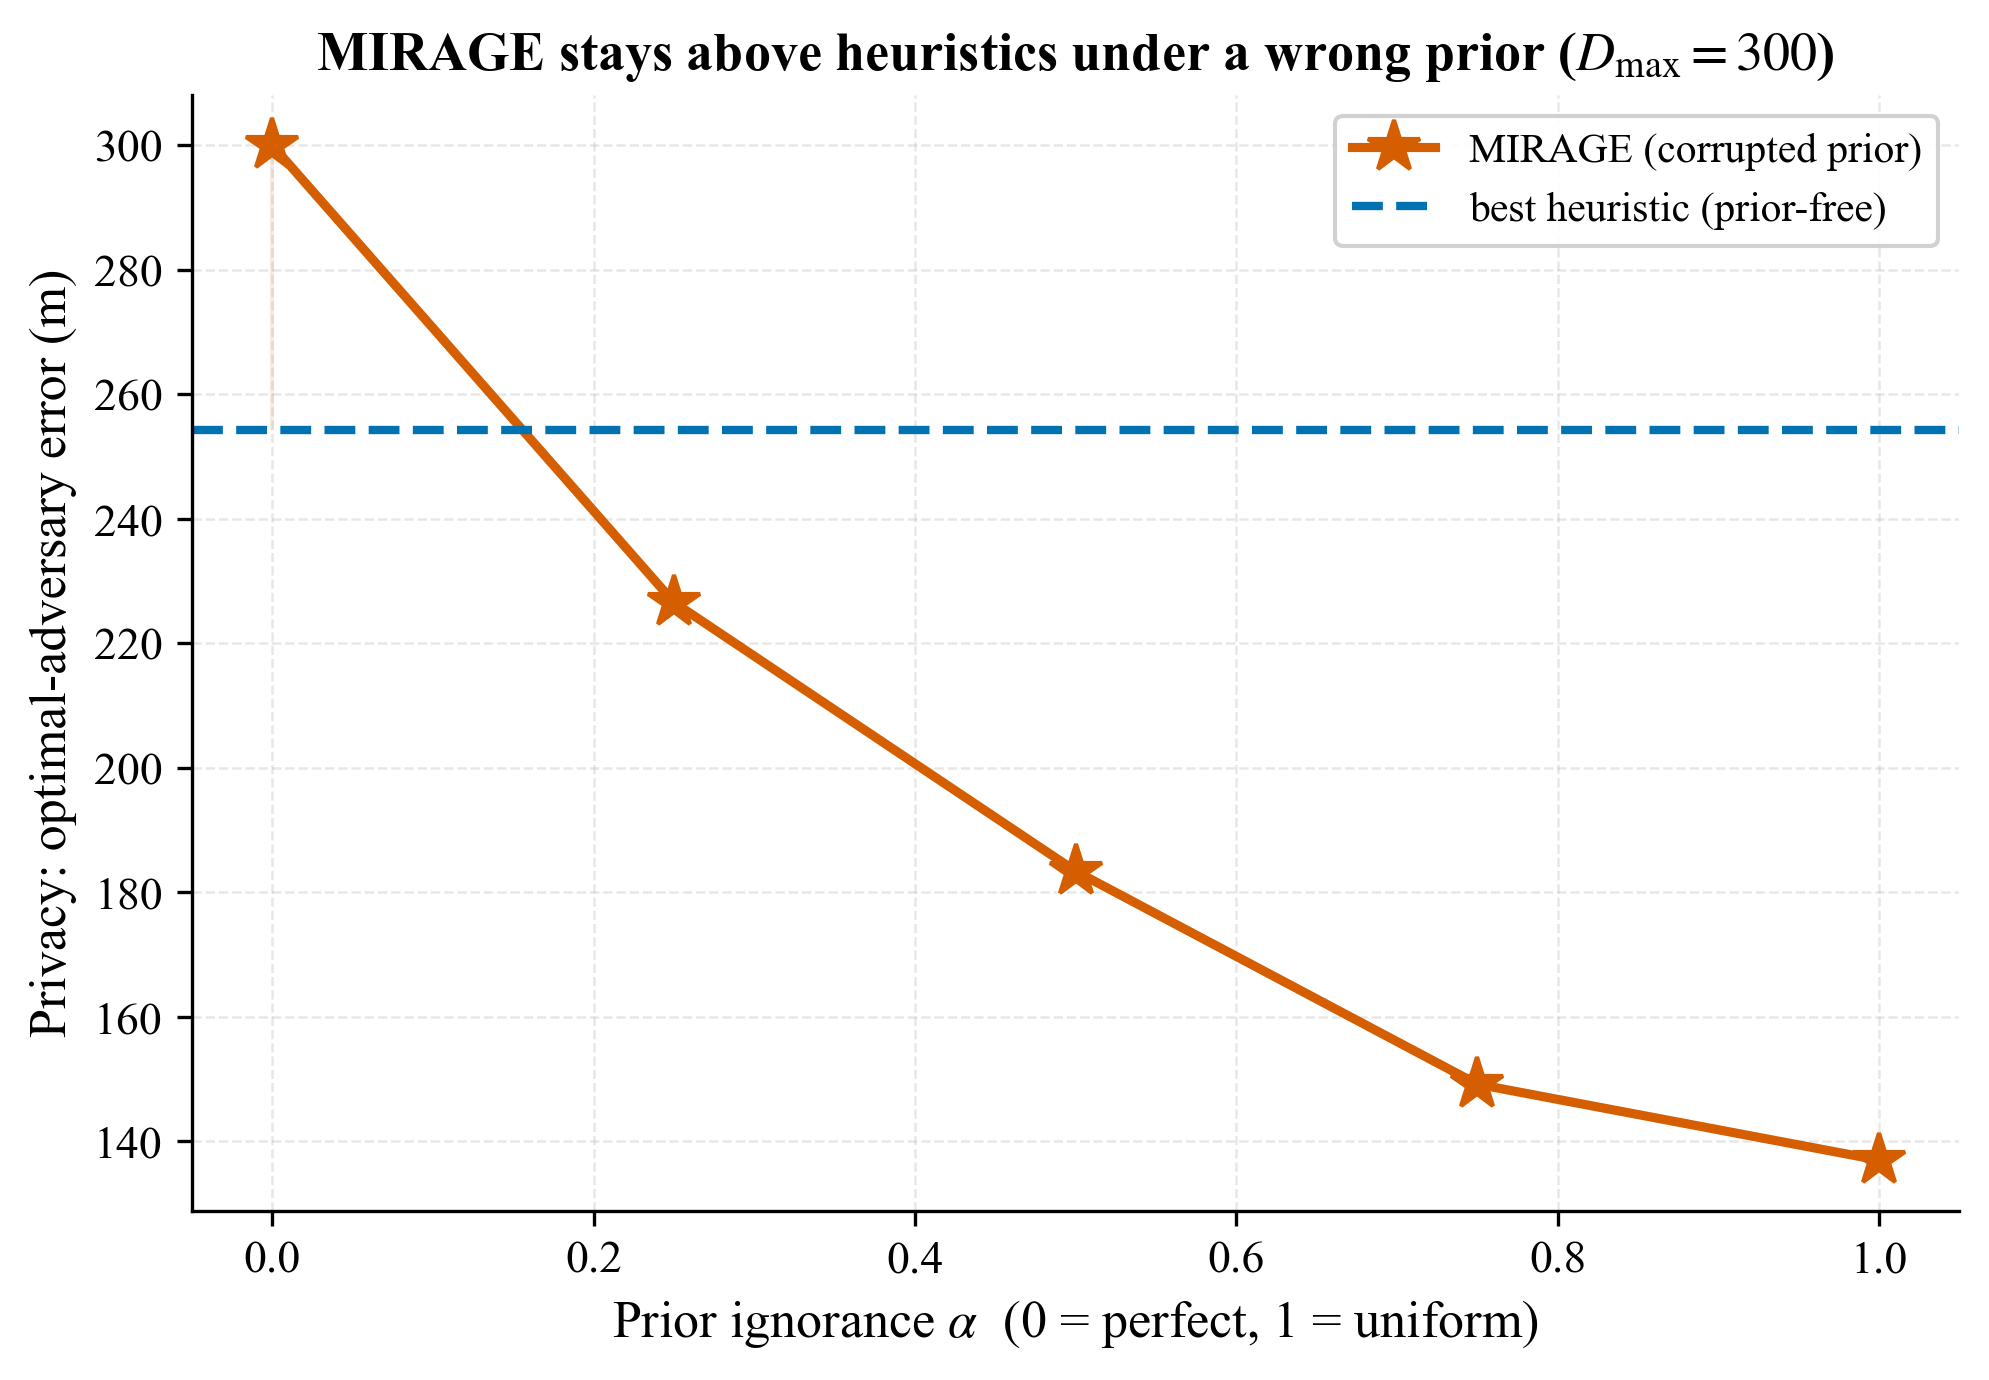
\includegraphics[width=0.85\linewidth]{fig_prior_robustness.png}
\caption{Robustness to prior misspecification. MIRAGE stays above the best
prior-free heuristic while the prior is reasonably accurate ($\alpha\lesssim0.25$);
a badly wrong prior can make it underperform.}
\label{fig:robust}
\end{figure}

% =====================================================================
\section{Results VI: Trajectory Adversary --- an Honest Limit}
\label{sec:traj}
% =====================================================================
MIRAGE is optimal against the snapshot adversary. Does that carry to the
trajectory adversary? We stress-test it, and the answer---honestly---is no, for an
instructive structural reason. Using the filtering adversary \eqref{eq:filter} on
real user traces (Fig.~\ref{fig:traj}), \emph{DP is the most trajectory-private
mechanism} at matched distortion: at $800$\,m distortion the tracking error is
$676$\,m for DP versus $\sim$$578$\,m for both MIRAGE variants. The cause is
MIRAGE's density-adaptive partition---the very device that makes it scalable and
snapshot-optimal. Because each release lies in a fixed region, \emph{observing it
reveals region membership}, which the sequential adversary exploits to localise;
DP's diffuse, unpartitioned noise leaks less across time.

Our trajectory-aware variant MIRAGE-T (per-step LP against the mobility-propagated
belief) helps, and instructively its benefit \emph{tracks mobility}. On stationary
GeoLife---where users linger, so the belief barely moves and the dynamic prior
$\approx$ the static one---MIRAGE-T essentially matches snapshot-MIRAGE
($\sim$$578$ vs.\ $577$\,m at $800$\,m distortion). On the mobile T-Drive taxis
(low self-transition), where the belief shifts each step and there is real
structure to exploit, MIRAGE-T improves trajectory privacy by $+9$ to $+13\%$ over
snapshot-MIRAGE at matched utility and \emph{nearly closes the gap to DP} ($624$
vs.\ $647$\,m at $800$\,m). So belief-aware release meaningfully helps exactly
where trajectory tracking is most dangerous, but does not fully overcome the
region-membership leak. This is a clean instance of the paper's thesis---privacy
is threat-model dependent, here even for an optimal mechanism---and it isolates the
key open problem: a \emph{scalable} graph mechanism jointly optimal against
snapshot and trajectory adversaries, plausibly via soft or overlapping regions
whose releases do not reveal membership.

\begin{figure}[t]\centering

\includegraphics[width=0.95\linewidth]{fig_trajectory_geolife_real.png}
\caption{Trajectory adversary (GeoLife, real traces). At matched distortion DP is
most trajectory-private; MIRAGE's region partition leaks membership, and the
mobility-aware MIRAGE-T does not close the gap.}
\label{fig:traj}
\end{figure}

\textbf{Can we un-leak the membership? A structural tension.} We tested the
natural fix directly: replace the single hard partition with a random
\emph{mixture} of two overlapping partitions, so a release can originate from
either partition's region and no longer reveals one region
(Fig.~\ref{fig:soft}). It helps only marginally---by $+2$ to $+7\%$ on the mobile
T-Drive traces and slightly \emph{hurts} on the stationary GeoLife ones---and in
neither case does it close the gap to DP (at $\sim$$800$\,m distortion,
$527$--$564$\,m for MIRAGE variants vs.\ $669$\,m for DP). The lesson is that the
tension is \emph{structural}: light de-partitioning is insufficient, because the
same local region structure that yields snapshot-optimality inherently
concentrates releases; matching DP's trajectory-robustness appears to require
genuinely diffuse support, which sacrifices the snapshot optimality. A mechanism
that is jointly optimal for both threats---perhaps a many-partition ensemble or a
continuous-support graph LP---remains the central open problem this analysis
sharpens.

\begin{figure}[t]\centering
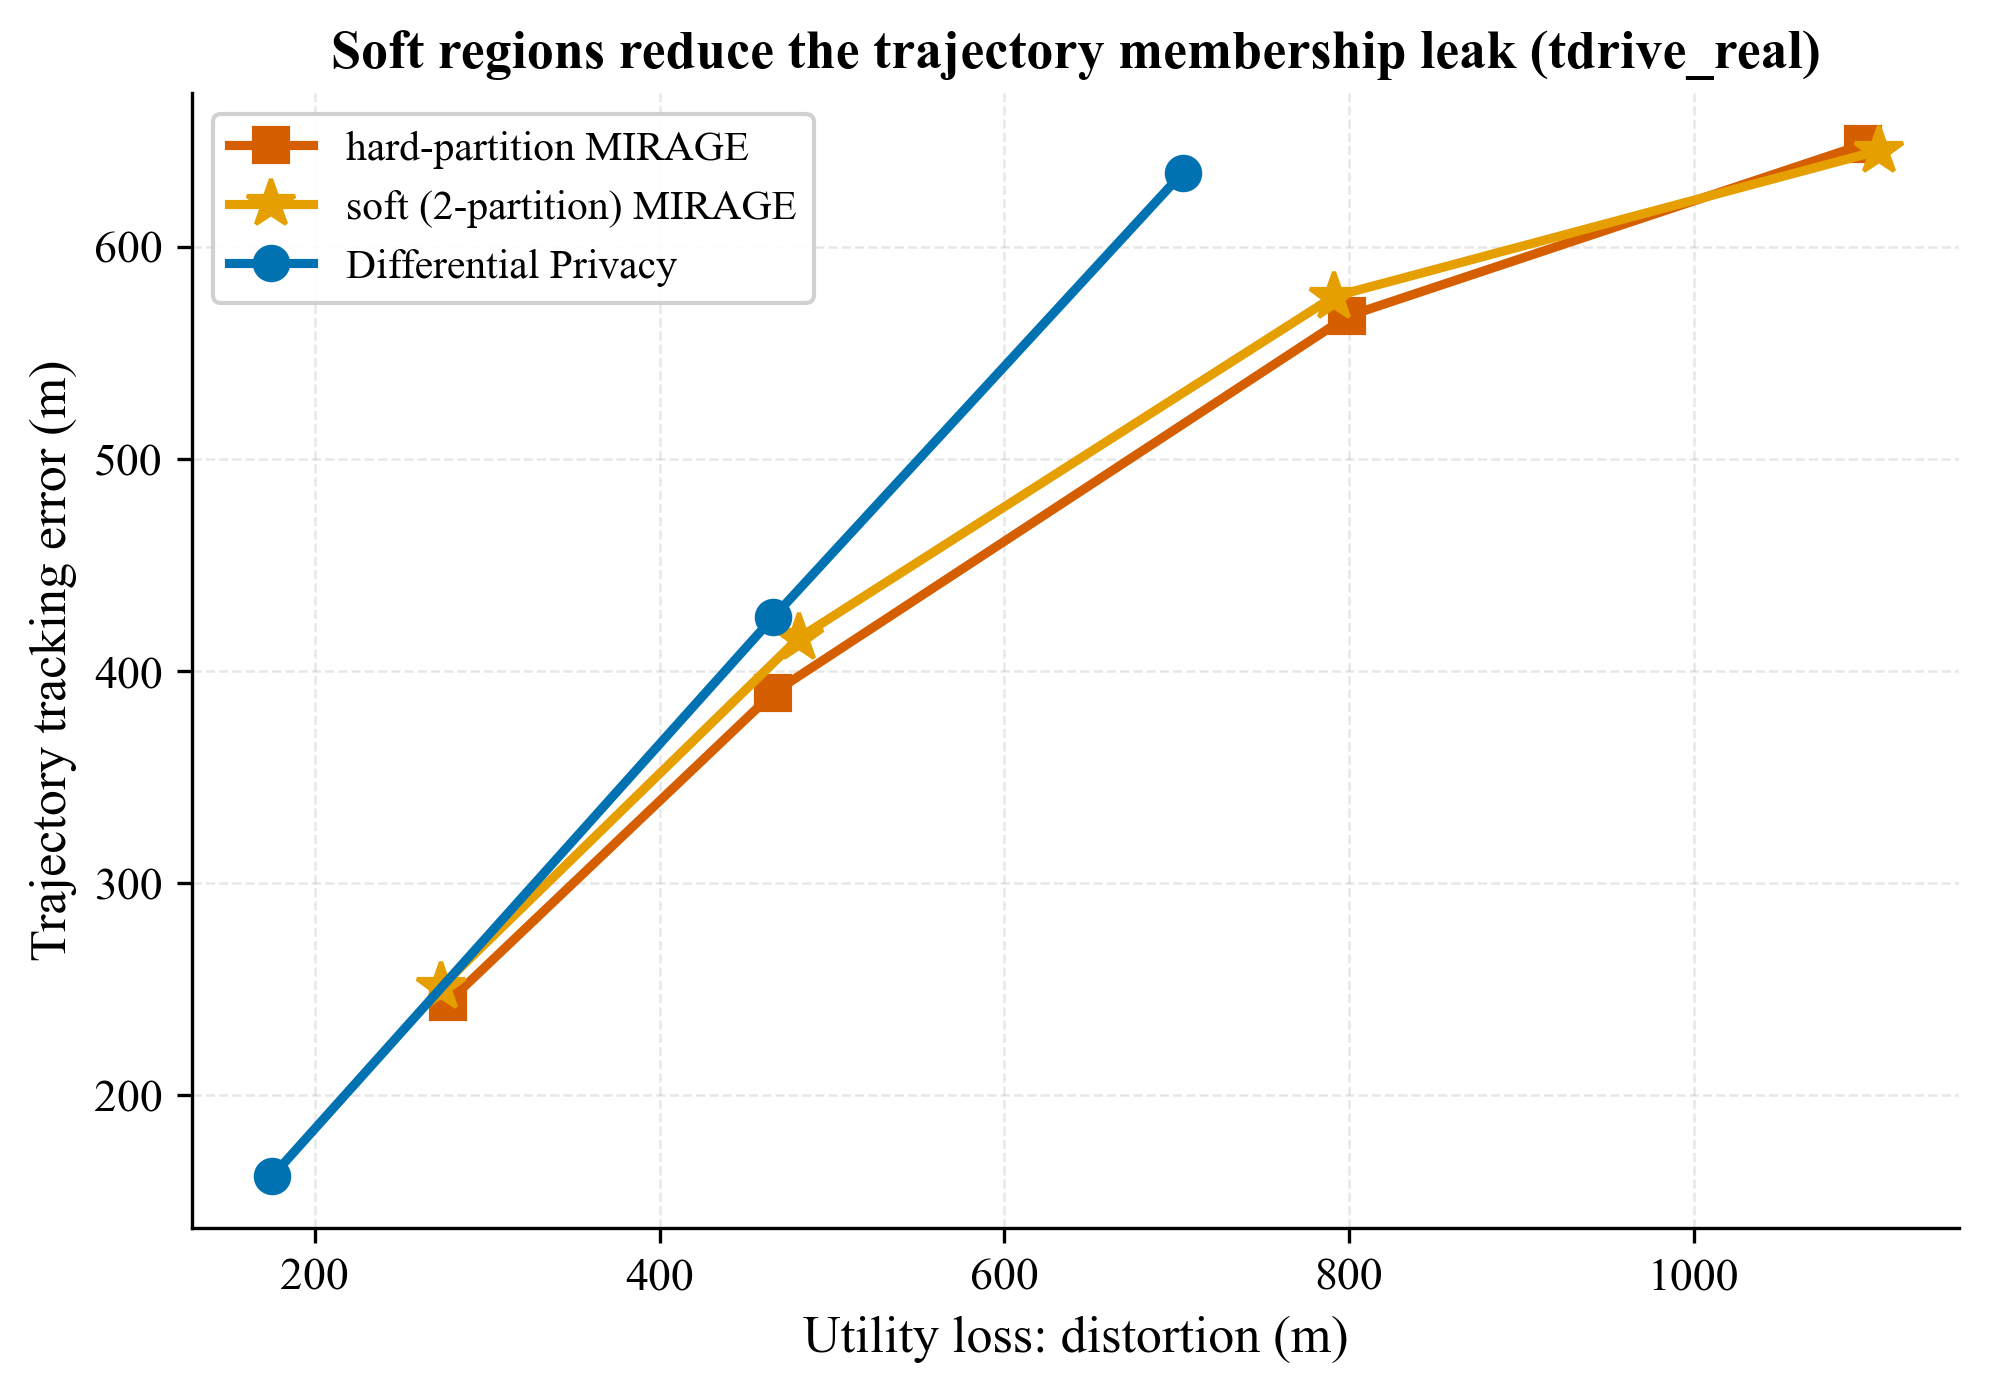
\includegraphics[width=0.85\linewidth]{fig_soft_region.png}
\caption{Attempting to close the trajectory gap with soft (two-partition) regions.
It helps marginally on mobile data and not at all on stationary data; DP remains
more trajectory-robust---the membership-leak tension is structural.}
\label{fig:soft}
\end{figure}

% =====================================================================
\section{Results VII: Energy-Model Sensitivity}
\label{sec:energy}
% =====================================================================
Per-report energy is $E=E_{\mathrm{radio}}+E_{\mathrm{comp}}+E_{\mathrm{retrans}}$,
with $E_{\mathrm{radio}}=P_{\mathrm{tx}}t_{\mathrm{tx}}$. Rather than fix one
radio, we sweep BLE, Zigbee, LoRa, NB-IoT, and LTE-M (Fig.~\ref{fig:energy}). The
common claim that radio transmission dominates holds only for LPWAN/cellular
radios ($99\%$ radio share for LoRa/NB-IoT/LTE-M) but \emph{not} for BLE, where
computation is $6$--$50\%$ of energy for BFS-based mechanisms. MIRAGE's
release-time cost is a single categorical draw ($O(1)$), so it is as
radio-dominated as DP; its LP cost is paid once, offline.

\begin{figure}[t]\centering
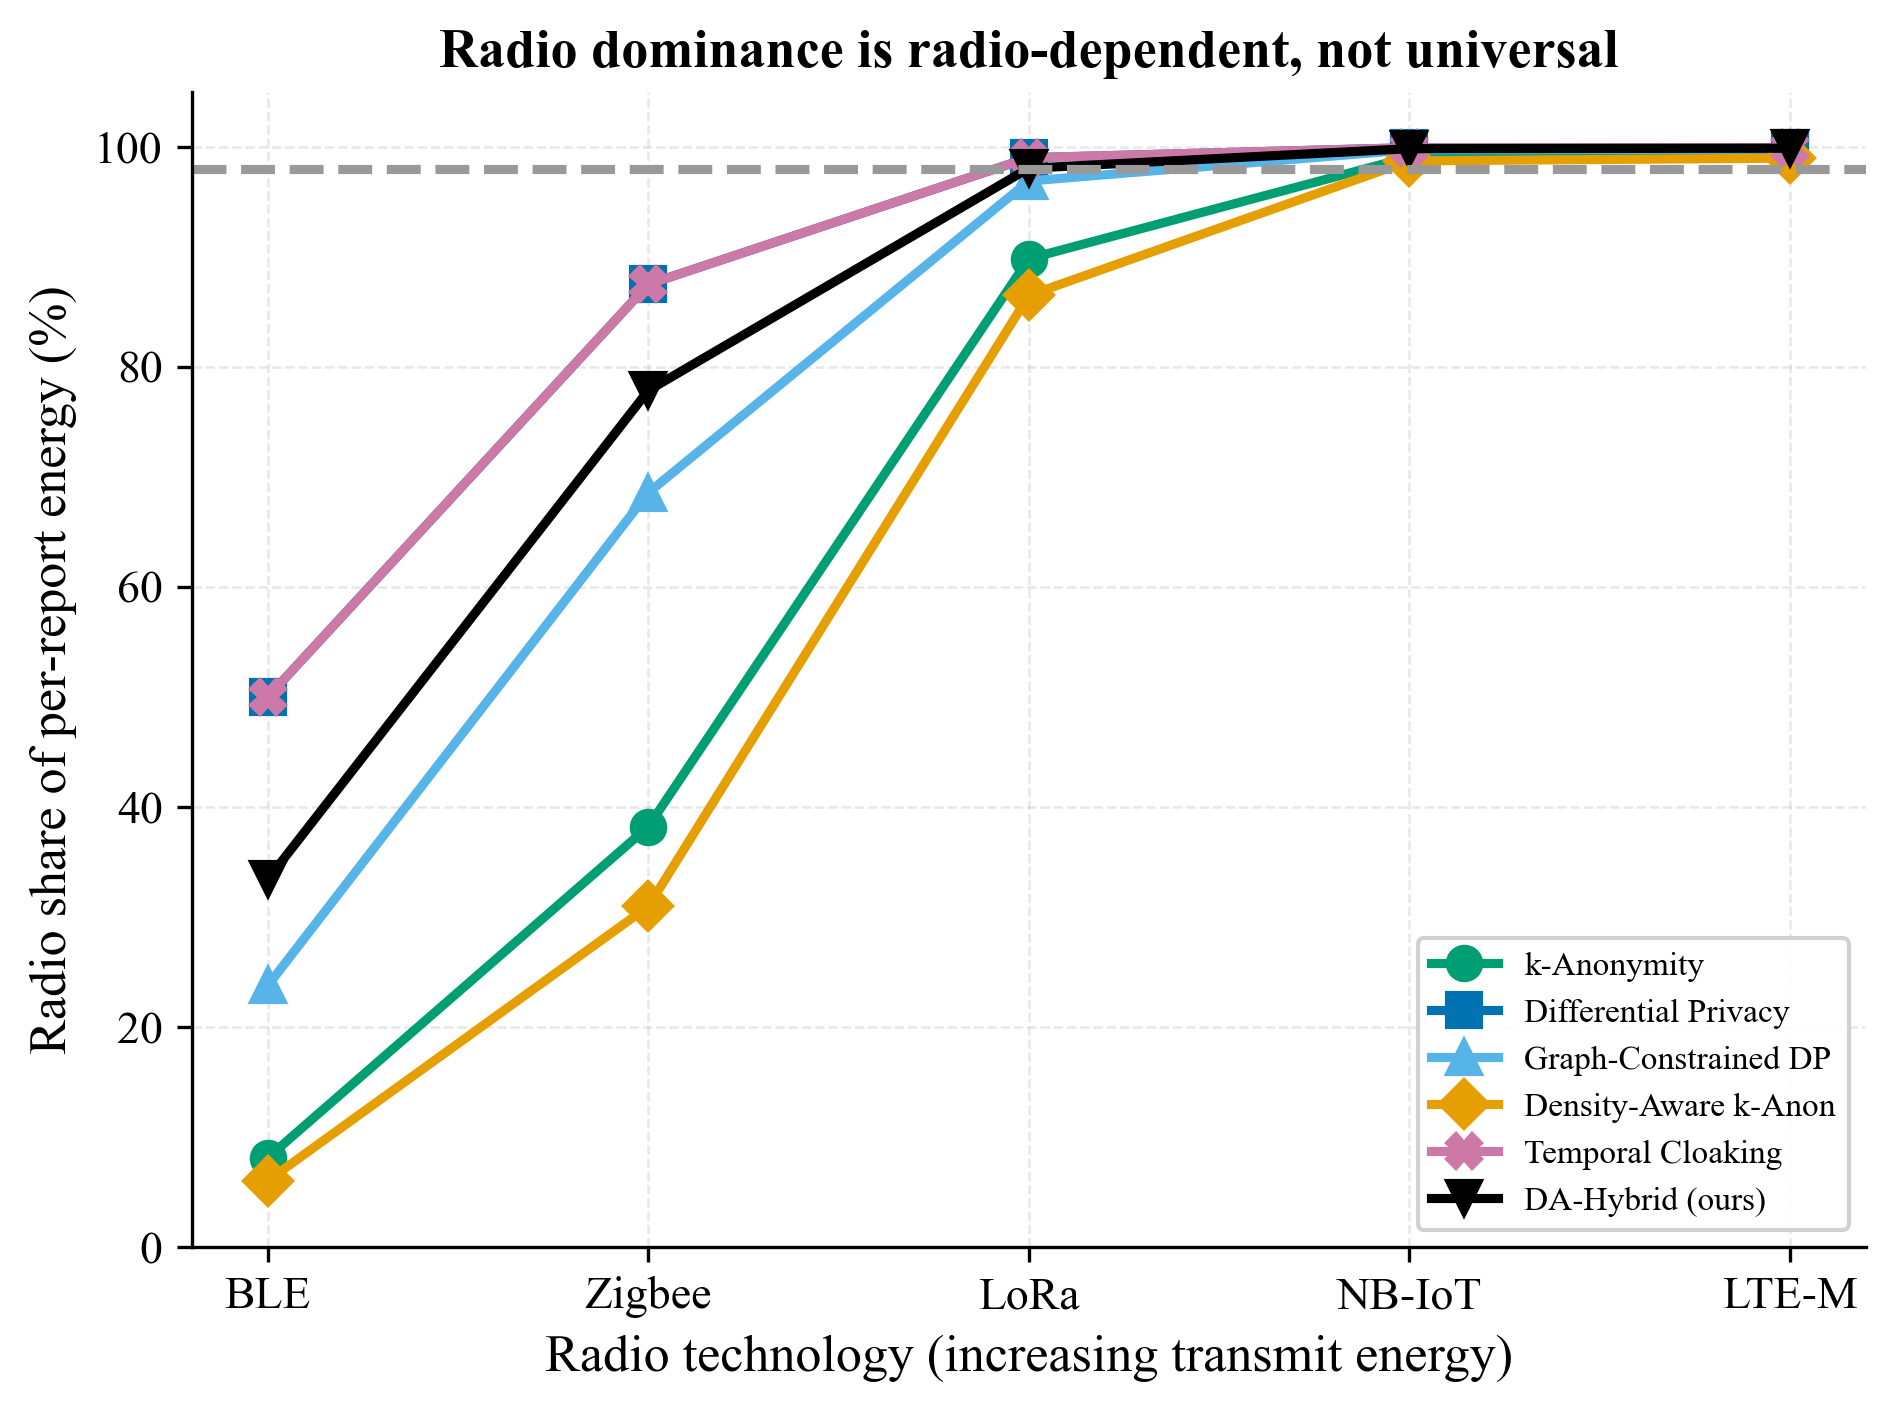
\includegraphics[width=0.95\linewidth]{fig_energy_sensitivity.png}
\caption{Radio share of per-report energy vs.\ radio technology. Radio dominance
is radio-dependent, not universal.}
\label{fig:energy}
\end{figure}

% =====================================================================
\section{Discussion}
\label{sec:discussion}
% =====================================================================
\textbf{Deployment guidance.} For a chosen utility budget on the operator's own
road network and mobility statistics, MIRAGE gives the release policy that
provably maximises snapshot-attacker error---up to $+22\%$ more privacy than tuned
heuristics at equal utility, with $100\%$ availability and on-graph outputs, and
the gain is largest where the population is spatially concentrated
(Section~\ref{sec:why}). Where a formal DP guarantee is required, the
geo-indistinguishability-constrained variant applies at a measured cost. Where
sequential tracking is the dominant threat, a diffuse mechanism (or the open
membership-hiding design of Section~\ref{sec:traj}) is preferable---the choice
must be made against the relevant adversary, which our two-threat metric makes
explicit.

\textbf{Threats to validity.} (i)~Absolute error is graph-granularity dependent,
so cross-\emph{topology} conclusions rest on adversary-privacy and availability,
not raw error. (ii)~The energy model is analytical, suited to ranking rather than
absolute prediction; we report its radio sensitivity explicitly. (iii)~The
mobility prior is first-order Markov; a richer prior would strengthen the
trajectory adversary and can only lower reported trajectory privacy---so our
trajectory numbers are, if anything, optimistic for all mechanisms. (iv)~The local
decomposition caps MIRAGE's reach at high distortion, where heuristics catch up at
the uncertainty ceiling; hierarchical regions would extend the advantage.
(v)~MIRAGE's optimality is prior-conditioned (Section~\ref{sec:robust}): a badly
misspecified prior can erase its advantage, so a deployer must estimate occupancy
reasonably well or use a distributionally-robust variant.

\textbf{Ethical use.} The framework is defensive: it helps operators release less
information for a given utility, and it exposes when a mechanism is weaker than its
nominal parameter suggests. The adversary models are standard and use only public
background knowledge.

% =====================================================================
\section{Conclusion and Future Work}
\label{sec:conclusion}
% =====================================================================
We measured location privacy on a common, adversary-grounded, threat-model-aware
scale, and brought optimal obfuscation to a real road network at city scale with
MIRAGE. On real networks of two cities across three datasets, deployed heuristics
leave $5$--$22\%$ of achievable privacy on the table in the practical regime,
while MIRAGE is Pareto-optimal with full availability and on-graph outputs; the
advantage is explained by prior heterogeneity, rankings hold from grid to real
topology, and availability is shown to be dataset-density-driven. We also showed,
honestly, that snapshot-optimality does not imply trajectory-optimality: the
scalability partition leaks region membership. The central open problem---a
scalable graph mechanism jointly optimal against snapshot and trajectory
adversaries via membership-hiding soft/overlapping regions---together with richer
mobility priors and hardware-measured energy, defines our future work. The
complete framework is released for reproducible extension.

% =====================================================================
\begin{thebibliography}{99}
% =====================================================================
\bibitem{sweeney2002} L.~Sweeney, ``$k$-Anonymity: A model for protecting
privacy,'' \emph{Int. J. Uncertainty, Fuzziness Knowl.-Based Syst.}, vol.~10,
no.~5, pp.~557--570, 2002.
\bibitem{gruteser2003} M.~Gruteser and D.~Grunwald, ``Anonymous usage of
location-based services through spatial and temporal cloaking,'' in \emph{Proc.
MobiSys}, 2003, pp.~31--42.
\bibitem{dwork2006} C.~Dwork, ``Differential privacy,'' in \emph{Proc. ICALP},
LNCS 4052, 2006, pp.~1--12.
\bibitem{shokri2011} R.~Shokri, G.~Theodorakopoulos, J.-Y.~Le Boudec, and
J.-P.~Hubaux, ``Quantifying location privacy,'' in \emph{Proc. IEEE S\&P}, 2011,
pp.~247--262.
\bibitem{shokri2012} R.~Shokri, G.~Theodorakopoulos, C.~Troncoso, J.-P.~Hubaux,
and J.-Y.~Le Boudec, ``Protecting location privacy: Optimal strategy against
localization attacks,'' in \emph{Proc. ACM CCS}, 2012, pp.~617--627.
\bibitem{shokri2015pets} R.~Shokri, ``Privacy games: Optimal user-centric data
obfuscation,'' \emph{Proc. Privacy Enhancing Technologies}, vol.~2015, no.~2,
pp.~299--315, 2015.
\bibitem{bordenabe2014} N.~E.~Bordenabe, K.~Chatzikokolakis, and C.~Palamidessi,
``Optimal geo-indistinguishable mechanisms for location privacy,'' in \emph{Proc.
ACM CCS}, 2014, pp.~251--262.
\bibitem{andres2013} M.~E.~Andr\'{e}s, N.~E.~Bordenabe, K.~Chatzikokolakis, and
C.~Palamidessi, ``Geo-indistinguishability: Differential privacy for
location-based systems,'' in \emph{Proc. ACM CCS}, 2013, pp.~901--914.
\bibitem{chatzikokolakis2013} K.~Chatzikokolakis \emph{et~al.}, ``Broadening the
scope of differential privacy using metrics,'' in \emph{Proc. PETS}, 2013,
pp.~82--102.
\bibitem{mokbel2006} M.~F.~Mokbel, C.-Y.~Chow, and W.~G.~Aref, ``The new Casper:
Query processing for location services without compromising privacy,'' in
\emph{Proc. VLDB}, 2006, pp.~763--774.
\bibitem{duckham2005} M.~Duckham and L.~Kulik, ``A formal model of obfuscation and
negotiation for location privacy,'' in \emph{Pervasive Computing}, LNCS 3468,
2005, pp.~152--170.
\bibitem{niu2014} B.~Niu, Q.~Li, X.~Zhu, G.~Cao, and H.~Li, ``Achieving
$k$-anonymity in privacy-aware location-based services,'' in \emph{Proc. IEEE
INFOCOM}, 2014, pp.~754--762.
\bibitem{xiao2015} Y.~Xiao and L.~Xiong, ``Protecting locations with differential
privacy under temporal correlations,'' in \emph{Proc. ACM CCS}, 2015,
pp.~1298--1309.
\bibitem{du2023} Y.~Du \emph{et~al.}, ``LDPTrace: Locally differentially private
trajectory synthesis,'' \emph{Proc. VLDB Endow.}, vol.~16, no.~8, pp.~1897--1909,
2023.
\bibitem{hu2024} Y.~Hu \emph{et~al.}, ``Real-time trajectory synthesis with local
differential privacy,'' in \emph{Proc. IEEE ICDE}, 2024, pp.~1685--1698.
\bibitem{buchholz2024} E.~Buchholz \emph{et~al.}, ``SoK: Can trajectory generation
combine privacy and utility?,'' \emph{Proc. PETS}, vol.~2024, no.~3, pp.~75--93,
2024.
\bibitem{zheng2009} Y.~Zheng, L.~Zhang, X.~Xie, and W.-Y.~Ma, ``Mining interesting
locations and travel sequences from GPS trajectories,'' in \emph{Proc. WWW}, 2009,
pp.~791--800.
\bibitem{zheng2008} Y.~Zheng, Q.~Li, Y.~Chen, X.~Xie, and W.-Y.~Ma, ``Understanding
mobility based on GPS data,'' in \emph{Proc. UbiComp}, 2008, pp.~312--321.
\end{thebibliography}
\end{document}
